\section*{CHƯƠNG 2. CƠ SỞ LÝ THUYẾT VÀ TỔNG QUAN TÀI LIỆU}
\addcontentsline{toc}{section}{\numberline{}CHƯƠNG 2. CƠ SỞ LÝ THUYẾT VÀ TỔNG QUAN TÀI LIỆU}
\setcounter{section}{2}
\setcounter{subsection}{0}
\setcounter{figure}{0}
\setcounter{table}{0}

\subsection*{2.1. Quy trình xử lý ảnh khuôn mặt trong thị giác máy tính}
\addcontentsline{toc}{subsection}{\numberline{}2.1. Quy trình xử lý ảnh khuôn mặt trong thị giác máy tính}

Trong các hệ thống thị giác máy tính phục vụ phân tích hành vi người dùng, quy trình tiền xử lý ảnh khuôn mặt đóng vai trò quyết định đến độ chính xác của các mô hình học sâu ở hạ nguồn. Một luồng xử lý chuẩn bao gồm ba bước cơ bản: phát hiện khuôn mặt, căn chỉnh hình học và kiểm soát chất lượng ảnh thu nhận.

\subsubsection*{2.1.1. Phát hiện khuôn mặt (Face Detection)}
\addcontentsline{toc}{subsubsection}{\numberline{}2.1.1. Phát hiện khuôn mặt (Face Detection)}

Phát hiện khuôn mặt là tác vụ xác định vị trí và kích thước của các khuôn mặt xuất hiện trong một khung hình tĩnh hoặc chuỗi video. Các thuật toán phát hiện hiện đại được chia thành hai nhóm chính:
\begin{itemize}
    \item \textbf{Phương pháp truyền thống (Haar Cascades, HOG):} Sử dụng các bộ trích xuất đặc trưng thủ công kết hợp bộ phân lớp tăng cường (AdaBoost) hoặc máy học vector hỗ trợ (SVM). Ưu điểm là tốc độ tính toán cực nhanh trên CPU, nhưng độ chính xác suy giảm mạnh khi đối mặt với góc quay nghiêng, khuôn mặt bị che khuất một phần hoặc điều kiện ánh sáng yếu.
    \item \textbf{Phương pháp học sâu (Single Shot MultiBox Detector - SSD, RetinaFace):} Mạng nơ-ron tích chập (CNN) phát hiện đồng thời hộp giới hạn (Bounding Box) và xác suất tồn tại khuôn mặt trên nhiều tầng tỷ lệ đặc trưng (Feature Pyramid Networks - FPN). Các mô hình như RetinaFace \cite{retinaface} đạt độ chính xác vượt trội nhờ khả năng dự đoán đồng thời 5 điểm mốc mốc hình học (mắt trái, mắt phải, đỉnh mũi, khóe miệng trái và khóe miệng phải), đáp ứng tốt yêu cầu triển khai trong môi trường bán lẻ thực tế.
\end{itemize}

\subsubsection*{2.1.2. Căn chỉnh khuôn mặt (Face Alignment)}
\addcontentsline{toc}{subsubsection}{\numberline{}2.1.2. Căn chỉnh khuôn mặt (Face Alignment)}

Ảnh khuôn mặt sau khi phát hiện thường bị nghiêng theo các trục xoay không gian (Roll, Pitch, Yaw). Quá trình căn chỉnh hình học thực hiện phép biến đổi affine (Affine Transformation) hai chiều nhằm xoay và chuẩn hóa khuôn mặt sao cho đường nối hai đồng tử mắt nằm ngang và tâm khuôn mặt được đưa về chính giữa khung hình chuẩn (kích thước $224 \times 224$ pixels). Phép biến đổi này giúp loại bỏ sự biến thiên do tư thế đầu của khách hàng, đảm bảo mô hình phân loại biểu cảm chỉ tập trung vào sự co giãn của các nhóm cơ mặt.

\subsubsection*{2.1.3. Đánh giá chất lượng ảnh thu nhận (Image Quality Assessment)}
\addcontentsline{toc}{subsubsection}{\numberline{}2.1.3. Đánh giá chất lượng ảnh thu nhận (Image Quality Assessment)}

Trong môi trường thực tế của cửa hàng, khách hàng liên tục di chuyển khiến nhiều khung hình bị mờ do chuyển động (motion blur), thiếu sáng hoặc quá sáng. Nếu đưa trực tiếp các khung hình suy biến này vào mô hình AI, kết quả dự đoán sẽ có độ bất định cao và gây nhiễu cho hệ thống phân tích. Do đó, em tích hợp bộ lọc chất lượng ảnh trước khi đưa vào pipeline nhận dạng biểu cảm, dựa trên ba yếu tố: độ mờ, độ sáng và độ tin cậy phát hiện khuôn mặt.

\begin{enumerate}
    \item \textbf{Phát hiện độ mờ bằng phương sai toán tử Laplace (Laplacian Variance):} Toán tử Laplace $\nabla^2$ là đạo hàm bậc hai phát hiện các vùng có cường độ sáng thay đổi đột ngột, tức các cạnh sắc nét trong ảnh. Ảnh sắc nét chứa nhiều cạnh rõ ràng nên phương sai lớn; ảnh mờ làm mất chi tiết cạnh nên phương sai nhỏ. Phương sai Laplace được tính theo công thức phương sai thống kê chuẩn \cite{gonzalez2018digital}:
    \begin{equation}
    \text{Var}_{\text{Lap}} = \frac{1}{M N} \sum_{x=1}^{M} \sum_{y=1}^{N} \left( \nabla^2 I(x, y) - \mu_{\text{Lap}} \right)^2
    \end{equation}
    Trong đó $\nabla^2 I(x, y) = \frac{\partial^2 I}{\partial x^2} + \frac{\partial^2 I}{\partial y^2}$ là toán tử Laplace 2D, $\mu_{\text{Lap}}$ là giá trị trung bình của ảnh sau khi qua bộ lọc Laplace, $M \times N$ là kích thước ảnh tính theo pixel.

    Giá trị $\text{Var}_{\text{Lap}}$ có miền giá trị từ $0$ đến vài nghìn tùy ảnh, trong khi điểm chất lượng tổng hợp $Q$ (trình bày bên dưới) yêu cầu tất cả các thành phần nằm trong đoạn $[0, 1]$ để các trọng số có ý nghĩa so sánh. Do đó, em chuẩn hóa bằng cách chia cho một ngưỡng bão hòa và chặn trên tại $1.0$:
    \begin{equation}
    S_{\text{blur}} = \min \left( \frac{\text{Var}_{\text{Lap}}}{300.0}, 1.0 \right)
    \end{equation}
    Ngưỡng $300.0$ được em lựa chọn dựa trên thực nghiệm: qua kiểm thử trên dữ liệu camera thu tại cửa hàng, các khuôn mặt đủ nét để nhận dạng biểu cảm cho $\text{Var}_{\text{Lap}}$ dao động trong khoảng $[200, 400]$. Em chọn $300$ --- trung điểm của khoảng này --- vì nếu đặt ngưỡng quá thấp (ví dụ $100$), ảnh còn khá mờ đã cho $S_{\text{blur}} = 1.0$, làm mất tác dụng lọc; ngược lại nếu đặt quá cao (ví dụ $1000$), hầu hết ảnh bình thường sẽ có điểm thấp, kéo lệch điểm tổng hợp $Q$.

    \item \textbf{Đánh giá phân bố độ sáng (Brightness Score):} Độ sáng trung bình $\mu_{\text{gray}}$ của vùng khuôn mặt là trung bình cộng tất cả giá trị pixel trên ảnh mức xám. Trên thang 8-bit, mỗi pixel có giá trị trong đoạn $[0, 255]$ ($0$ là đen tuyệt đối, $255$ là trắng tuyệt đối), nên mức cân bằng sáng lý tưởng nằm tại trung điểm $\frac{0 + 255}{2} = 127.5$. Em đo mức độ lệch khỏi điểm cân bằng này và chuẩn hóa về $[0, 1]$:
    \begin{equation}
    S_{\text{bright}} = \max \left( 0.0, 1.0 - \frac{|\mu_{\text{gray}} - 127.5|}{127.5} \right)
    \end{equation}
    Trong công thức trên: $|\mu_{\text{gray}} - 127.5|$ là độ lệch tuyệt đối so với mức cân bằng; chia cho $127.5$ (độ lệch cực đại, xảy ra khi $\mu_{\text{gray}} = 0$ hoặc $255$) để chuẩn hóa về $[0, 1]$; lấy $1.0$ trừ đi để đảo chiều --- ảnh cân bằng sáng cho điểm cao ($S_{\text{bright}} = 1.0$ khi $\mu_{\text{gray}} = 127.5$), ảnh quá tối hoặc quá sáng cho điểm thấp ($S_{\text{bright}} = 0.0$ khi $\mu_{\text{gray}} = 0$ hoặc $255$). Các con số $127.5$ trong công thức không phải tham số tự chọn mà là hệ quả trực tiếp của thang đo 8-bit.
\end{enumerate}

Điểm số chất lượng tổng hợp $Q$ được tính bằng trung bình có trọng số của ba thành phần:
\begin{equation}
Q = 0.45 \cdot C_{\text{face}} + 0.35 \cdot S_{\text{blur}} + 0.20 \cdot S_{\text{bright}}
\end{equation}
Em phân bổ trọng số dựa trên mức độ ảnh hưởng của từng yếu tố đến chất lượng nhận dạng biểu cảm: $C_{\text{face}}$ (độ tin cậy phát hiện khuôn mặt) nhận trọng số lớn nhất $0.45$ vì nếu mô hình không chắc chắn có khuôn mặt trong khung hình thì mọi phân tích biểu cảm tiếp theo đều vô nghĩa; $S_{\text{blur}}$ nhận $0.35$ vì ảnh mờ làm mất các đặc trưng co giãn cơ mặt --- yếu tố cốt lõi để phân biệt các biểu cảm; $S_{\text{bright}}$ nhận $0.20$ vì mô hình học sâu có khả năng chịu đựng sự lệch sáng ở mức vừa phải, chỉ cần loại bỏ khi ảnh quá tối hoặc cháy sáng hoàn toàn. Tổng ba trọng số bằng $1.0$ đảm bảo $Q \in [0, 1]$. Khung hình chỉ được chấp nhận khi $Q \ge 0.45$ và $C_{\text{face}} \ge 0.70$. Các khung hình không đạt chuẩn bị loại bỏ và ghi nhận lý do cụ thể (\textit{IMAGE\_BLURRY, IMAGE\_TOO\_DARK, IMAGE\_TOO\_BRIGHT}).

\subsection*{2.2. Lý thuyết nhận dạng biểu cảm khuôn mặt (Facial Expression Recognition - FER)}
\addcontentsline{toc}{subsection}{\numberline{}2.2. Lý thuyết nhận dạng biểu cảm khuôn mặt (Facial Expression Recognition - FER)}

\subsubsection*{2.2.1. Hệ thống phân loại biểu cảm cơ bản theo Paul Ekman}
\addcontentsline{toc}{subsubsection}{\numberline{}2.2.1. Hệ thống phân loại biểu cảm cơ bản theo Paul Ekman}

Theo nghiên cứu kinh điển của nhà tâm lý học Paul Ekman và Hệ thống mã hóa hành động cơ mặt (Facial Action Coding System - FACS) \cite{facs}, con người có 6 biểu cảm cơ bản mang tính phổ quát toàn cầu không phụ thuộc vào văn hóa và chủng tộc, kết hợp với trạng thái trung tính để tạo thành \textbf{7 lớp biểu cảm chuẩn}:
\begin{enumerate}
    \item \textbf{Vui vẻ (Happy):} Đặc trưng bởi cơ gò má kéo khóe miệng lên trên và cơ vòng mi làm híp mắt (nụ cười Duchenne).
    \item \textbf{Buồn bã (Sad):} Khóe miệng trễ xuống, đầu trong lông mày nhướng lên và mí mắt trên sụp xuống.
    \item \textbf{Tức giận (Angry):} Hai lông mày hạ thấp và kéo sát lại gần nhau, ánh mắt nhìn chằm chằm, môi mím chặt.
    \item \textbf{Sợ hãi (Fear):} Lông mày nhướng cao và kéo lại gần nhau, mí mắt trên mở rộng, miệng hé mở căng thẳng.
    \item \textbf{Ngạc nhiên (Surprise):} Lông mày cong vút lên cao, mắt mở to tròn, hàm dưới trễ xuống làm mở rộng khoang miệng.
    \item \textbf{Ghê sợ / Khó chịu (Disgust):} Mũi nhăn lại, môi trên kéo cao lên làm lộ răng trên.
    \item \textbf{Trung tính (Neutral):} Các cơ mặt ở trạng thái thả lỏng, không có biến dạng cơ học rõ rệt.
\end{enumerate}

\subsubsection*{2.2.2. Kiến trúc mạng nơ-ron tích chập (CNN) trong bài toán FER}
\addcontentsline{toc}{subsubsection}{\numberline{}2.2.2. Kiến trúc mạng nơ-ron tích chập (CNN) trong bài toán FER}

Bài toán FER được mô hình hóa dưới dạng bài toán phân lớp đa lớp (Multi-class Classification). Ảnh khuôn mặt sau khi được phát hiện, căn chỉnh và chuẩn hóa sẽ được đưa vào mạng nơ-ron tích chập để trích xuất đặc trưng không gian ở nhiều mức độ khác nhau. Các lớp tích chập đầu thường học các đặc trưng cơ bản như cạnh, vùng sáng tối và đường cong; các lớp sâu hơn kết hợp những đặc trưng này thành cấu trúc có ý nghĩa hơn như mắt, lông mày, khóe miệng, nếp nhăn vùng mũi hoặc độ mở của miệng. Từ các đặc trưng đó, lớp phân loại cuối cùng sinh ra phân bố xác suất cho 7 lớp biểu cảm tiêu chuẩn.

Trong thực tế, các kiến trúc mạng học sâu hiện đại thường kết hợp các khối tích chập sâu, kỹ thuật học chuyển giao (Transfer Learning) từ các mô hình được tiền huấn luyện trên những tập dữ liệu khuôn mặt quy mô lớn (như VGGFace2, MS-Celeb-1M, AffectNet, FER2013 \cite{fer2013}) và đôi khi bổ sung cơ chế chú ý (Attention Mechanisms) để tập trung vào các vùng mặt có giá trị phân biệt cao. Một số kiến trúc thường gặp gồm:
\begin{itemize}
    \item \textbf{MobileNetV2 / MobileNetV3 \cite{mobilenetv2}:} Sử dụng các khối tích chập tách biệt theo chiều sâu (Depthwise Separable Convolutions) và cấu trúc đảo ngược nút cổ chai (Inverted Residuals). Kiến trúc này giúp giảm đáng kể số lượng tham số và số phép tính dấu phẩy động (FLOPs), cho phép triển khai suy luận với tốc độ trên 30 FPS trên các máy chủ phổ thông hoặc thiết bị biên.
    \item \textbf{ResNet:} Sử dụng các kết nối tắt (Residual Connections) để hỗ trợ huấn luyện mạng CNN có nhiều lớp. Trong quá trình lan truyền ngược, gradient là tín hiệu cho biết mỗi trọng số của mô hình cần được điều chỉnh theo hướng nào để làm giảm hàm mất mát. Khi mô hình có quá nhiều lớp, tín hiệu này có thể nhỏ dần khi truyền từ lớp cuối về các lớp đầu, khiến trọng số ở các lớp tích chập đầu cập nhật rất chậm hoặc gần như không được cập nhật; hiện tượng đó được gọi là triệt tiêu gradient (Vanishing Gradient). ResNet khắc phục một phần vấn đề này bằng cách cộng trực tiếp đầu vào của một khối với đầu ra sau các lớp tích chập, thường được mô tả dưới dạng $y = F(x) + x$. Nhờ đường truyền tắt này, thông tin và gradient có thể lan truyền ổn định hơn qua nhiều lớp, giúp mô hình CNN cập nhật trọng số hiệu quả hơn và học được các đặc trưng khuôn mặt phức tạp hơn phục vụ phân loại biểu cảm.
    \item \textbf{EfficientNet:} Không tập trung chủ yếu vào kết nối tắt như ResNet, mà tối ưu sự cân bằng giữa độ sâu, độ rộng của mạng và độ phân giải ảnh đầu vào thông qua chiến lược mở rộng đồng bộ (Compound Scaling). Cách thiết kế này giúp cải thiện hiệu quả tính toán, đạt độ chính xác tốt với số tham số và FLOPs hợp lý. Trong bài toán FER, EfficientNet phù hợp khi cần cân bằng giữa chất lượng phân loại biểu cảm và chi phí suy luận, đặc biệt với dữ liệu khuôn mặt có biến thiên về ánh sáng, góc nhìn và kích thước khuôn mặt.
\end{itemize}

Đối với FER, các kiến trúc CNN sâu có lợi thế vì biểu cảm khuôn mặt nhiều khi chỉ khác nhau ở các thay đổi rất nhỏ, chẳng hạn khóe miệng hơi nhếch, lông mày hơi cau, mí mắt hơi hạ hoặc vùng mũi nhăn nhẹ. Tuy nhiên, việc sử dụng mạng càng sâu không tự động bảo đảm kết quả tốt hơn; hiệu quả thực tế còn phụ thuộc vào chất lượng dữ liệu huấn luyện, cân bằng lớp, tiền xử lý khuôn mặt, khả năng chống nhiễu và độ trễ trong quá trình suy luận khi triển khai camera thời gian thực.

\subsubsection*{2.2.3. Đầu ra của mạng nơ-ron trong bài toán FER}
\addcontentsline{toc}{subsubsection}{\numberline{}2.2.3. Đầu ra của mạng nơ-ron trong bài toán FER}

Sau khi mạng CNN trích xuất đặc trưng khuôn mặt, lớp phân loại cuối cùng tạo ra đầu ra thô cho từng lớp biểu cảm. Đầu ra này được biểu diễn dưới dạng vector logits $\bm{z} = [z_1, z_2, \dots, z_7]^T \in \mathbb{R}^7$. Hàm kích hoạt Softmax chuyển đổi vector logits thành phân bố xác suất hợp lệ trên 7 lớp biểu cảm:
\begin{equation}
p_i = \frac{e^{z_i}}{\sum_{j=1}^{7} e^{z_j}}, \quad \forall i \in \{1, 2, \dots, 7\}, \quad \text{sao cho} \quad \sum_{i=1}^{7} p_i = 1.0
\end{equation}
Mô hình được tối ưu hóa bằng hàm mất mát Cross-Entropy:
\begin{equation}
\mathcal{L}_{\text{CE}} = - \sum_{i=1}^{7} y_i \log(p_i)
\end{equation}
Trong đó $\bm{y}$ là vector nhãn one-hot thực tế. Lớp có xác suất lớn nhất $p_{\text{max}} = \max_i(p_i)$ được chọn làm biểu cảm chủ đạo (Dominant Expression), và giá trị $p_{\text{max}}$ chính là độ tin cậy dự đoán (Confidence).

\subsubsection*{2.2.4. Quy trình thực nghiệm lựa chọn detector và mô hình FER}
\addcontentsline{toc}{subsubsection}{\numberline{}2.2.4. Quy trình thực nghiệm lựa chọn detector và mô hình FER}

Trong bài toán phân tích biểu cảm từ camera, mô hình FER không nhận trực tiếp toàn bộ khung hình video. Mỗi khung hình trước hết phải đi qua bước phát hiện và căn chỉnh khuôn mặt để xác định vùng mặt hợp lệ. Sau đó, vùng mặt đã được chuẩn hóa mới được đưa vào bộ phân loại biểu cảm. Vì vậy, việc lựa chọn mô hình cần được thực hiện theo chuỗi phụ thuộc:
\begin{center}
\textit{Khung hình video $\rightarrow$ detector/căn chỉnh khuôn mặt $\rightarrow$ mô hình FER $\rightarrow$ xác suất 7 lớp biểu cảm.}
\end{center}

Nếu detector bỏ sót khuôn mặt, phát hiện sai vùng mặt hoặc căn chỉnh lệch, đầu vào của mô hình FER sẽ bị nhiễu và kết quả phân loại biểu cảm không còn đáng tin cậy. Do đó, trong đồ án này em không chỉ khảo sát mô hình FER mà còn cần đánh giá riêng bước phát hiện/căn chỉnh khuôn mặt, sau đó đánh giá tổ hợp detector và FER trong cùng điều kiện.

Việc đánh giá trong đồ án này được thực hiện bằng chương trình benchmark tự chạy. Chương trình trước hết lưu dự đoán của từng mẫu vào tệp CSV, sau đó đọc chính các tệp dự đoán này để tính Accuracy, Macro-F1, Detection Rate và các phân vị độ trễ. Bảng LaTeX và biểu đồ PNG được sinh tự động từ kết quả tính toán; em không nhập thủ công các giá trị trong bảng và không dùng số liệu công bố bên ngoài để xếp hạng.

Lần thực nghiệm có thể chạy lại hiện tại sử dụng CK+ Extended \cite{lucey2010ckplus}. Từ 920 ảnh xám $48 \times 48$ pixel, em chỉ lấy 182 mẫu thuộc hai phần \textit{PublicTest} và \textit{PrivateTest}, đồng thời loại lớp \textit{contempt} để thống nhất đầu ra bảy lớp. Vì CK+ trong lần thử này gồm các ảnh khuôn mặt đã được crop, ảnh được phóng lên $224 \times 224$ pixel trước khi chạy detector. Việc phóng ảnh chỉ nhằm tránh giới hạn kích thước đầu vào tối thiểu và không tạo thêm chi tiết khuôn mặt.

Ở bước phát hiện khuôn mặt, em chạy OpenCV, MTCNN và RetinaFace trên cùng 182 mẫu, cùng máy và cùng quy trình đo thời gian. Kết quả do chương trình sinh ra được trình bày trong Bảng~\ref{tab:ckplus-detector-benchmark}.

\begin{table}[H]
    \centering
    \caption{Kết quả benchmark detector do chương trình sinh ra trên 182 mẫu CK+}
    \label{tab:ckplus-detector-benchmark}
    \small
    \resizebox{\textwidth}{!}{\begin{tabular}{lrrrr}
\hline
Detector & Detection Rate & False Positive & Exact Count & p95 (ms) \\
\hline
opencv & 1.0000 & 0.0000 & 1.0000 & 24.61 \\
mtcnn & 1.0000 & 0.0000 & 1.0000 & 356.58 \\
retinaface & 1.0000 & 0.0000 & 1.0000 & 1119.50 \\
\hline
\end{tabular}
}
\end{table}

\begin{figure}[H]
    \centering
    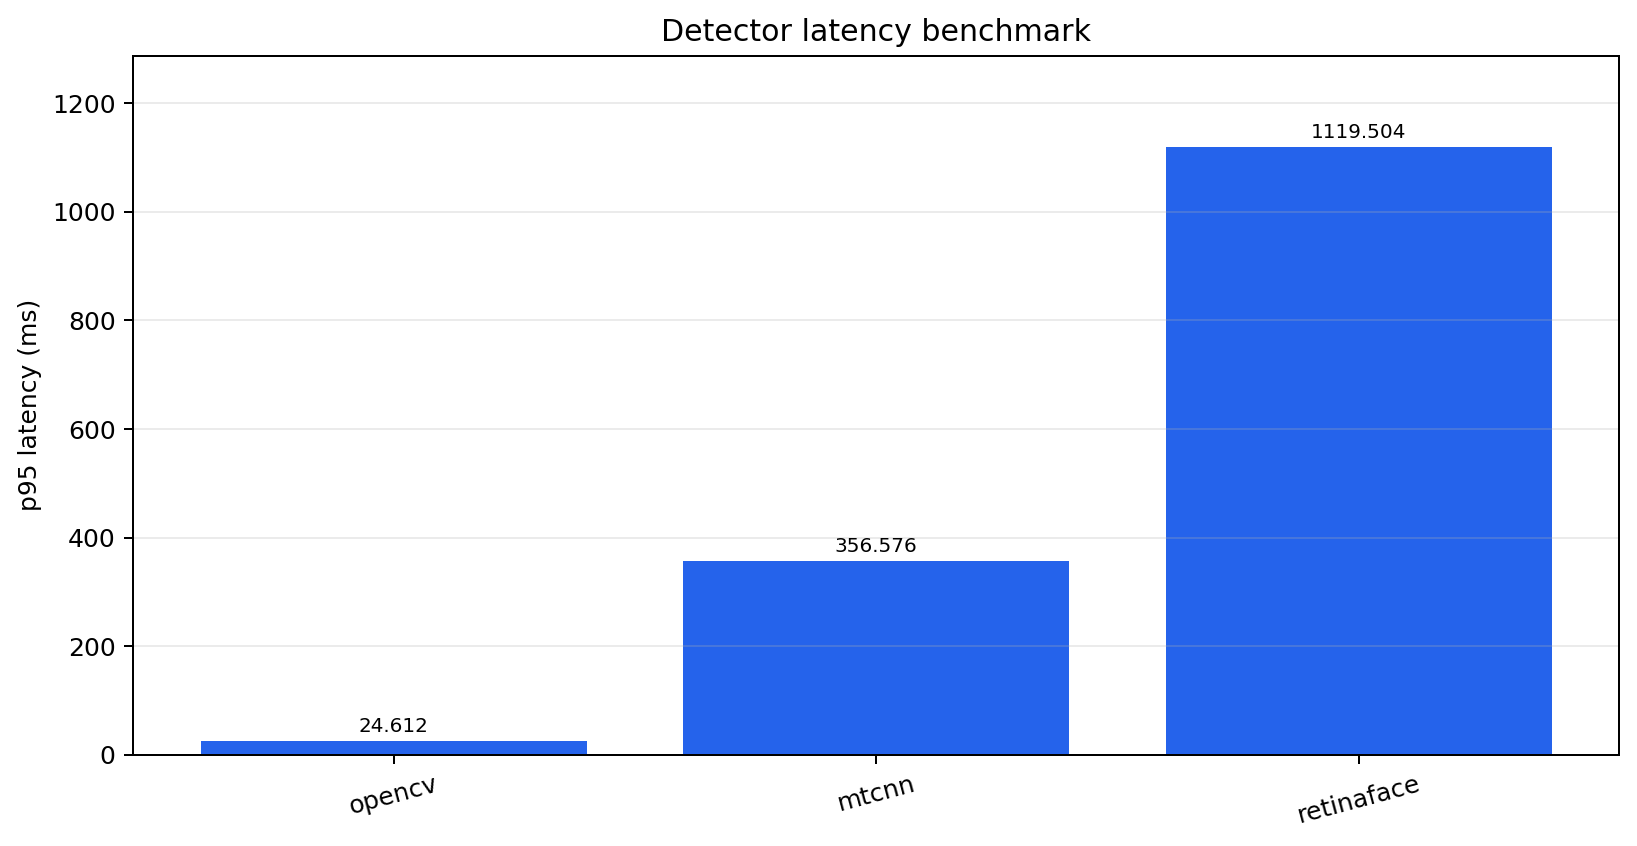
\includegraphics[width=0.82\textwidth]{../../fer-benchmark/outputs/detector_comparison.png}
    \caption{So sánh độ trễ p95 của ba detector từ lần chạy benchmark}
    \label{fig:ckplus-detector-benchmark}
\end{figure}

\textbf{Ý nghĩa của kết quả so sánh detector.} Detection Rate cho biết tỷ lệ ảnh có khuôn mặt mà detector tìm thấy được ít nhất một khuôn mặt. Exact Count phản ánh tỷ lệ ảnh mà số khuôn mặt phát hiện được đúng bằng số khuôn mặt mong đợi. Trong lần thử này, cả ba detector đều đạt Detection Rate và Exact Count bằng 1,0000, nghĩa là OpenCV, MTCNN và RetinaFace đều phát hiện đúng một khuôn mặt trên toàn bộ 182 ảnh. No Result chưa xuất hiện ở bước này vì không có ảnh nào bị bỏ sót.

Khi khả năng phát hiện trên tập kiểm thử đang bằng nhau, độ trễ trở thành tiêu chí phân biệt trực tiếp. Chỉ số p95 biểu thị rằng 95\% số mẫu có thời gian xử lý không vượt quá giá trị được ghi trong bảng. OpenCV đạt p95 bằng 24,61 ms, MTCNN đạt 356,58 ms và RetinaFace đạt 1119,50 ms. Như vậy, trên cùng phần cứng và cùng dữ liệu, MTCNN cần thời gian xử lý lớn hơn OpenCV khoảng 14,5 lần, còn RetinaFace lớn hơn khoảng 45,5 lần. Kết quả này cho thấy việc dùng detector phức tạp hơn không tạo thêm lợi ích về tỷ lệ phát hiện trên bộ ảnh CK+ đã crop, nhưng làm tăng đáng kể thời gian xử lý.

CK+ không chứa ảnh âm, tức ảnh không có khuôn mặt, nên cột False Positive bằng 0 chỉ có nghĩa là tập dữ liệu không tạo ra trường hợp để đo phát hiện nhầm. Giá trị này không chứng minh rằng detector sẽ không nhận nhầm vật thể thành khuôn mặt trong môi trường cửa hàng. Trong phạm vi thử nghiệm hiện tại, Bảng~\ref{tab:ckplus-detector-benchmark} được dùng để lựa chọn detector có cùng khả năng phát hiện nhưng có độ trễ thấp hơn; vì vậy em lựa chọn OpenCV cho bước xử lý tiếp theo.

\textbf{Lý do sử dụng thư viện DeepFace trong thực nghiệm.} Ở bước phân loại biểu cảm, em sử dụng thư viện DeepFace vì thư viện cung cấp sẵn quy trình nhận ảnh khuôn mặt, chuẩn hóa đầu vào và trả về xác suất của bảy lớp biểu cảm gồm \textit{angry}, \textit{disgust}, \textit{fear}, \textit{happy}, \textit{sad}, \textit{surprise} và \textit{neutral}. Tập nhãn này phù hợp trực tiếp với cấu trúc dữ liệu cảm xúc của hệ thống. DeepFace cũng cho phép thay đổi detector bằng cùng một tham số cấu hình, nhờ đó OpenCV, MTCNN và RetinaFace có thể được chạy trong cùng một quy trình mà không phải viết ba luồng xử lý khác nhau. Điều này giúp hạn chế sai lệch do cách tiền xử lý và tạo điều kiện so sánh các detector trong cùng điều kiện.

Trong lần thử này, DeepFace nạp mạng CNN bảy lớp thông qua mô-đun \texttt{EmotionClient} và tệp trọng số tiền huấn luyện \path{facial_expression_model_weights.h5}. Việc sử dụng trọng số tiền huấn luyện giúp em xây dựng được mốc đánh giá ban đầu mà không phải tự huấn luyện lại mạng từ đầu. Khi bỏ qua detector và đưa trực tiếp 182 ảnh khuôn mặt CK+ vào mạng CNN, chương trình đo được Accuracy bằng 0,6264, Macro-F1 bằng 0,3834 và độ trễ suy luận p95 bằng 3,68 ms. Accuracy cho biết tỷ lệ dự đoán đúng trên toàn bộ mẫu, còn Macro-F1 tính F1 riêng cho từng lớp rồi lấy trung bình, do đó phản ánh rõ hơn khả năng nhận diện đồng đều giữa bảy lớp khi dữ liệu bị mất cân bằng. Kết quả này được dùng làm mốc của bộ phân loại cảm xúc đang sử dụng trước khi đánh giá toàn bộ pipeline.

Để đo ảnh hưởng của bước phát hiện và căn chỉnh lên kết quả cuối, em tiếp tục ghép cùng mạng CNN bảy lớp với từng detector. Mỗi lỗi không trả ra khuôn mặt được tính là một mẫu không có kết quả, thay vì bị loại khỏi phép tính. Bảng~\ref{tab:ckplus-e2e-benchmark} và Hình~\ref{fig:ckplus-e2e-benchmark} đều được xuất trực tiếp từ lần chạy này.

\begin{table}[H]
    \centering
    \caption{Kết quả benchmark end-to-end do chương trình sinh ra trên 182 mẫu CK+}
    \label{tab:ckplus-e2e-benchmark}
    \small
    \resizebox{\textwidth}{!}{\begin{tabular}{lrrrr}
\hline
Tổ hợp & Detection Rate & Macro-F1 & No Result & p95 (ms) \\
\hline
opencv + CNN FER 7-class & 1.0000 & 0.3328 & 0.0000 & 29.27 \\
mtcnn + CNN FER 7-class & 1.0000 & 0.2867 & 0.0000 & 361.02 \\
retinaface + CNN FER 7-class & 1.0000 & 0.3249 & 0.0000 & 1126.42 \\
\hline
\end{tabular}
}
\end{table}

\begin{figure}[H]
    \centering
    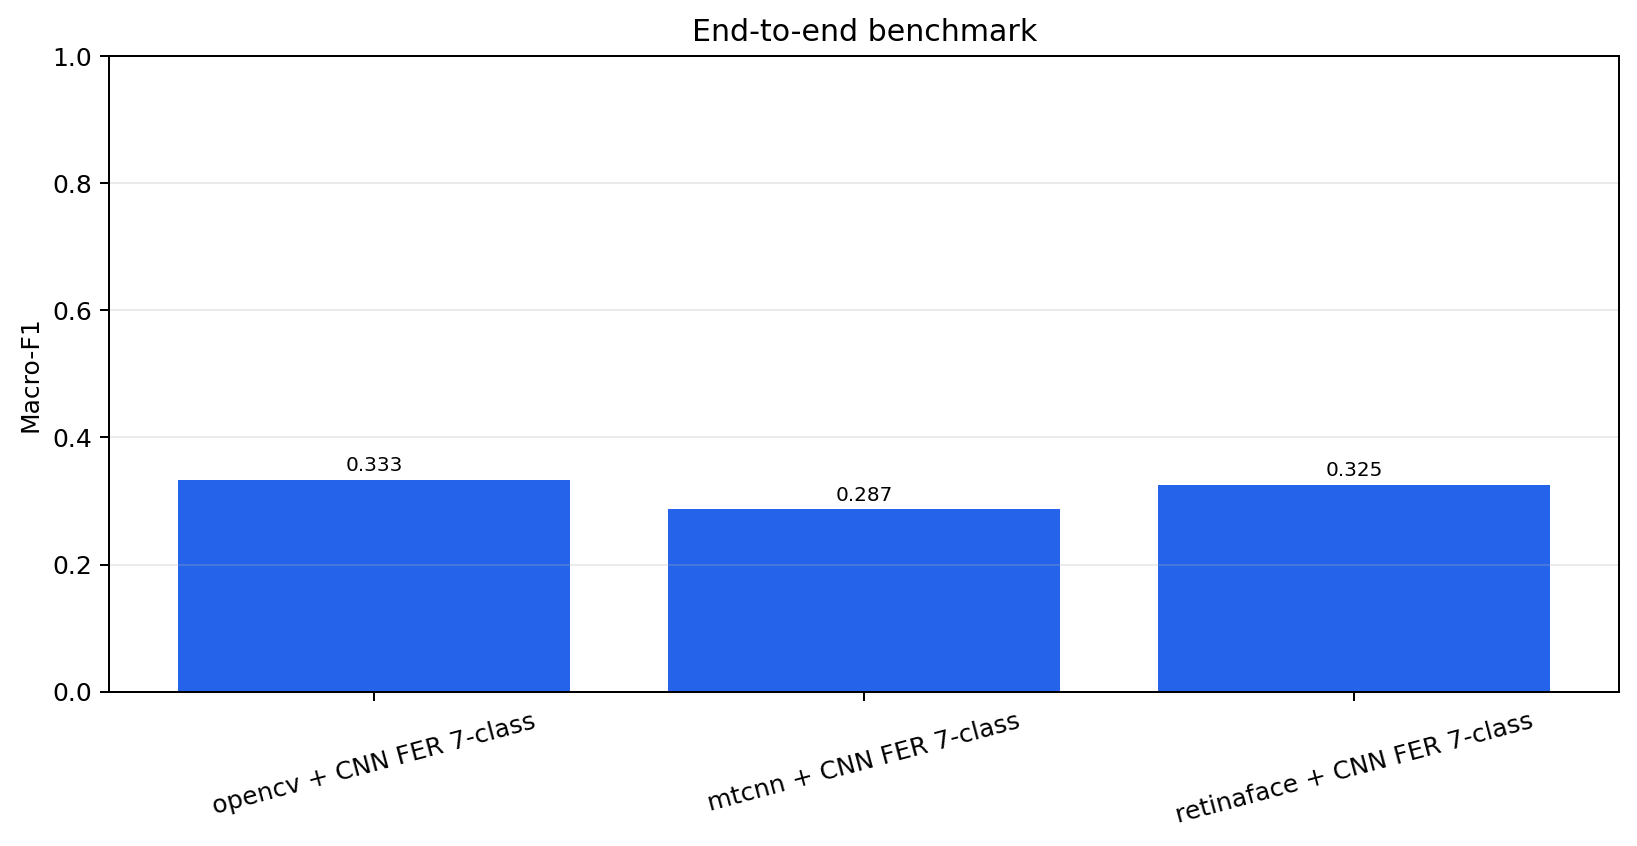
\includegraphics[width=0.9\textwidth]{../../fer-benchmark/outputs/end_to_end_comparison.png}
    \caption{So sánh Macro-F1 end-to-end của các tổ hợp từ lần chạy benchmark}
    \label{fig:ckplus-e2e-benchmark}
\end{figure}

\textbf{Ý nghĩa của kết quả end-to-end.} Bảng~\ref{tab:ckplus-e2e-benchmark} không chỉ đo khả năng tìm thấy khuôn mặt mà đo kết quả sau toàn bộ chuỗi xử lý: phát hiện khuôn mặt, crop/căn chỉnh vùng mặt và phân loại biểu cảm. Detection Rate bằng 1,0000 và No Result bằng 0,0000 ở cả ba tổ hợp cho thấy mọi ảnh đều đi qua được toàn bộ pipeline và đều nhận được một nhãn biểu cảm. Tuy nhiên, No Result bằng 0 không có nghĩa là tất cả dự đoán đều đúng; độ chính xác phân loại phải được xem qua Accuracy và Macro-F1.

Kết quả cho thấy tổ hợp OpenCV và mạng CNN bảy lớp đạt Macro-F1 cao nhất, bằng 0,3328, đồng thời có Accuracy bằng 0,6099 và độ trễ p95 thấp nhất, bằng 29,27 ms. Tổ hợp MTCNN đạt Macro-F1 bằng 0,2867 với p95 bằng 361,02 ms; tổ hợp RetinaFace đạt Macro-F1 bằng 0,3249 với p95 bằng 1126,42 ms. Sự khác nhau về Macro-F1 xuất hiện dù cả ba detector đều tìm thấy khuôn mặt, bởi mỗi detector tạo ra vùng crop và kết quả căn chỉnh khác nhau. Vùng mặt được cắt quá rộng, quá hẹp hoặc thay đổi vị trí của mắt, mũi và miệng sẽ làm thay đổi đầu vào của mạng CNN, từ đó ảnh hưởng đến xác suất biểu cảm cuối cùng.

Như vậy, hai bảng phục vụ hai quyết định liên tiếp. Bảng~\ref{tab:ckplus-detector-benchmark} cho thấy OpenCV có khả năng phát hiện tương đương hai detector còn lại nhưng nhanh hơn rõ rệt. Bảng~\ref{tab:ckplus-e2e-benchmark} tiếp tục cho thấy lợi thế tốc độ của OpenCV không làm giảm kết quả phân loại; ngược lại, tổ hợp dùng OpenCV còn đạt Macro-F1 cao nhất trong ba tổ hợp. Trên cơ sở đồng thời xem xét khả năng phát hiện, chất lượng phân loại và độ trễ trong quá trình suy luận, em lựa chọn tổ hợp OpenCV và mạng CNN bảy lớp cho pipeline hiện tại.

Macro-F1 bằng 0,3328 vẫn là kết quả thấp và thấp hơn đáng kể so với Accuracy bằng 0,6099. Nguyên nhân chính là tập kiểm thử mất cân bằng mạnh, trong đó lớp \textit{neutral} chiếm 119/182 mẫu, trong khi các lớp \textit{fear}, \textit{sad} và \textit{disgust} có rất ít mẫu. Mô hình có thể dự đoán đúng nhiều ảnh \textit{neutral} và tạo ra Accuracy tương đối cao, nhưng nhận diện kém các lớp ít mẫu nên Macro-F1 bị giảm. Vì vậy, kết quả lựa chọn OpenCV ở đây phản ánh phương án phù hợp nhất trong các tổ hợp đã chạy trên CK+ đã crop, chứ chưa khẳng định chất lượng phân loại biểu cảm đã đáp ứng hoàn toàn môi trường bán lẻ thực tế.

Để kết luận mô hình phù hợp nhất cho camera cửa hàng, bước thực nghiệm tiếp theo vẫn phải bổ sung tập ảnh/video camera có nhãn, gồm cả ảnh không có khuôn mặt, mặt nhỏ, mặt nghiêng, che khuất, mờ và thay đổi ánh sáng; đồng thời chạy nhiều mô hình FER trên cùng vùng mặt do detector đã chọn tạo ra. Khi chưa có các tệp dự đoán đó, em không gắn kết luận ``tối ưu'' cho EfficientFace, DAN, POSTER++ hoặc ResEmoteNet. Quy tắc lựa chọn cuối cùng là loại các phương án không đạt ngưỡng Detection Rate và p95, sau đó ưu tiên Macro-F1 end-to-end; Accuracy chỉ dùng làm chỉ số bổ sung vì dữ liệu FER thường mất cân bằng lớp.

\subsection*{2.3. Khó khăn khi xử lý chuỗi cảm xúc video và các phương pháp khắc phục}
\addcontentsline{toc}{subsection}{\numberline{}2.3. Khó khăn khi xử lý chuỗi cảm xúc video và các phương pháp khắc phục}

Ở phần trước, đầu ra của mô hình FER được mô tả trên từng ảnh hoặc từng khung hình đơn lẻ. Tuy nhiên, trong kịch bản video hoặc camera thời gian thực, hệ thống không xử lý một ảnh độc lập mà xử lý một chuỗi khung hình liên tục theo thời gian. Vì vậy, vấn đề chính không chỉ là mô hình dự đoán đúng trên một khung hình, mà còn là làm sao để chuỗi kết quả cảm xúc ổn định, ít bị nhiễu và có thể tổng hợp thành thông tin trải nghiệm có ý nghĩa.

\subsubsection*{2.3.1. Kết quả FER không ổn định theo từng khung hình}
\addcontentsline{toc}{subsubsection}{\numberline{}2.3.1. Khó khăn: kết quả FER không ổn định theo từng khung hình}

Khi phân tích video, nếu mỗi khung hình được xử lý độc lập và nhãn có xác suất cao nhất được lấy trực tiếp làm kết quả cuối cùng, chuỗi cảm xúc có thể dao động liên tục. Ví dụ, một khách hàng đang có biểu cảm vui vẻ có thể bị nhận nhầm thành ngạc nhiên trong một vài khung hình khi đang nói chuyện, mở miệng hoặc quay đầu. Tương tự, ánh sáng thay đổi, khuôn mặt bị che khuất một phần, ảnh bị mờ hoặc góc nhìn nghiêng cũng có thể làm xác suất giữa các lớp biểu cảm thay đổi đột ngột.

Hiện tượng này được gọi là nhấp nháy ở mức khung hình (Frame-level Flickering). Về mặt nghiệp vụ, nếu dùng trực tiếp kết quả từng khung hình để đánh giá trải nghiệm khách hàng, dashboard có thể hiển thị trạng thái thay đổi quá nhanh và dữ liệu tổng hợp có thể bị lệch bởi các dự đoán nhiễu ngắn hạn. Do đó, hệ thống cần cơ chế xử lý theo thời gian để giảm tác động của các biến động nhất thời. Dưới đây là một vài phương pháp thường được sử dụng để khắc phục vấn đề này

\subsubsection*{2.3.2. Làm mịn kết quả ở mức khung hình bằng EMA}
\addcontentsline{toc}{subsubsection}{\numberline{}2.3.2. Làm mịn kết quả ở mức khung hình bằng EMA}

Một phương pháp khắc phục là không làm mịn trực tiếp nhãn cảm xúc, mà làm mịn vector xác suất đầu ra của mô hình FER. Trong đồ án, kỹ thuật Trung bình trượt hàm mũ (Exponential Moving Average - EMA) được áp dụng như một bước hậu xử lý sau mô hình nhận dạng biểu cảm. EMA không thay thế mô hình FER, mà giúp chuỗi xác suất đầu ra ổn định hơn trước khi chọn biểu cảm chủ đạo.

Gọi $\bm{p}_t = [p_t^{(1)}, \dots, p_t^{(7)}]^T$ là vector xác suất đầu ra của mô hình tại khung hình thứ $t$, và $\bm{s}_t = [s_t^{(1)}, \dots, s_t^{(7)}]^T$ là vector xác suất đã làm mịn. Công thức cập nhật đệ quy được định nghĩa:
\begin{equation}
\bm{s}_t = \alpha \cdot \bm{p}_t + (1 - \alpha) \cdot \bm{s}_{t-1}
\end{equation}
Trong đó $\alpha \in (0, 1]$ là hệ số làm mịn (Smoothing Factor). Nếu $\alpha$ lớn, kết quả phản ứng nhanh hơn với khung hình mới nhưng dễ bị ảnh hưởng bởi nhiễu tức thời. Nếu $\alpha$ nhỏ, kết quả ổn định hơn nhưng phản ứng chậm hơn khi biểu cảm thật sự thay đổi. Với kịch bản camera thời gian thực, giá trị $\alpha$ thường được chọn ở mức trung bình để cân bằng giữa độ ổn định và khả năng phản ứng.

Sau khi có vector $\bm{s}_t$, biểu cảm chủ đạo tại thời điểm $t$ được xác định bằng lớp có xác suất đã làm mịn lớn nhất. Ngoài ra, hệ thống chỉ nên tổng hợp phiên khi đã có đủ số lượng khung hình hợp lệ tối thiểu ($N_{\text{frames}} \ge N_{\text{min}}$), nhằm tránh kết luận từ quá ít dữ liệu quan sát.

\subsubsection*{2.3.3. Tổng hợp kết quả ở mức phiên trải nghiệm}
\addcontentsline{toc}{subsubsection}{\numberline{}2.3.3. Tổng hợp kết quả ở mức phiên trải nghiệm}

Sau khi chuỗi xác suất đã được làm mịn, hệ thống cần tổng hợp các kết quả rời rạc thành dữ liệu cấp phiên. Một phiên trải nghiệm có thể được hiểu là khoảng thời gian khách hàng xuất hiện tại một khu vực hoặc một điểm chạm cụ thể, chẳng hạn khu vực chờ, quầy tư vấn hoặc quầy thanh toán. Thay vì lưu một kết luận riêng lẻ cho từng khung hình, hệ thống tổng hợp các kết quả đã làm mịn để xác định biểu cảm chủ đạo, tỷ lệ biểu cảm tích cực/tiêu cực và xu hướng thay đổi cảm xúc trong phiên.

Bên cạnh biểu cảm chủ đạo, sự chuyển dịch cảm xúc theo thời gian cũng là thông tin quan trọng. Ví dụ, chuỗi kết quả có thể chuyển từ trung tính sang vui vẻ sau khi khách hàng được tư vấn, hoặc từ trung tính sang căng thẳng tại khu vực chờ nếu thời gian chờ kéo dài. Bằng cách theo dõi trạng thái cảm xúc chủ đạo sau làm mịn qua các cửa sổ thời gian liên tiếp, hệ thống có thể xây dựng ma trận chuyển dịch cảm xúc (\textit{Expression Transition Matrix}):
\begin{equation}
T_{i \to j} = P(\text{State}_{t+1} = j \mid \text{State}_t = i)
\end{equation}
Trong đó $T_{i \to j}$ biểu diễn xác suất trạng thái cảm xúc chuyển từ lớp $i$ ở thời điểm hiện tại sang lớp $j$ ở thời điểm kế tiếp. Một tỷ lệ chuyển dịch cao từ $\text{Neutral} \to \text{Happy}$ tại quầy tư vấn có thể gợi ý trải nghiệm tư vấn tích cực hơn, trong khi chuyển dịch từ $\text{Neutral} \to \text{Angry}$ hoặc $\text{Neutral} \to \text{Sad}$ tại quầy thu ngân có thể là tín hiệu cần kiểm tra lại quy trình phục vụ. Các kết luận này không nên được hiểu là đánh giá tuyệt đối về tâm lý khách hàng, mà là chỉ báo thống kê hỗ trợ phân tích trải nghiệm.

\subsection*{2.4. Lý thuyết quản trị trải nghiệm khách hàng (Customer Experience - CX) trong bán lẻ}
\addcontentsline{toc}{subsection}{\numberline{}2.4. Lý thuyết quản trị trải nghiệm khách hàng (Customer Experience - CX) trong bán lẻ}

Sau khi hệ thống đã có thể nhận dạng biểu cảm và xử lý chuỗi kết quả theo thời gian, bước tiếp theo là chuyển các kết quả kỹ thuật đó thành thông tin nghiệp vụ có ý nghĩa. Đối với bài toán phân tích trải nghiệm khách hàng tại cửa hàng bán lẻ, biểu cảm khuôn mặt không nên được xem như kết luận tuyệt đối về tâm lý khách hàng, mà được sử dụng như một tín hiệu quan sát để hỗ trợ đánh giá trải nghiệm tại từng điểm chạm. Vì vậy, trong phần này, em sẽ trình bày cơ sở lý thuyết về quản trị trải nghiệm khách hàng, mô hình hành trình khách hàng trong cửa hàng, cách suy luận trạng thái trải nghiệm từ nhiều tín hiệu và các chỉ số định lượng phục vụ cho việc  xây dựng dashboard CRM.

\subsubsection*{2.4.1. Mô phỏng hành trình khách hàng đa điểm chạm (Customer Journey Touchpoints)}
\addcontentsline{toc}{subsubsection}{\numberline{}2.4.1. Mô hình hành trình khách hàng đa điểm chạm (Customer Journey Touchpoints)}

Trong cửa hàng bán lẻ, khách hàng thường đi qua nhiều khu vực khác nhau trong suốt quá trình mua sắm. Có thể mô tả hành trình này dưới dạng chuỗi các điểm chạm liên tiếp:
\begin{center}
$\text{Cổng vào} \xrightarrow{\text{Zone 1}} \text{Khu chờ} \xrightarrow{\text{Zone 2}} \text{Quầy tư vấn} \xrightarrow{\text{Zone 3}} \text{Khu sản phẩm} \xrightarrow{\text{Zone 4}} \text{Quầy thanh toán} \xrightarrow{\text{Zone 5}} \text{Cổng ra}$
\end{center}
Mỗi khu vực đảm nhiệm một vai trò khác nhau trong quá trình phục vụ khách hàng, nên thời gian khách hàng dừng lại ở từng khu vực cũng không giống nhau. Khi kết quả cảm xúc được gắn với khu vực tương ứng, doanh nghiệp có thêm cơ sở để đánh giá chất lượng trải nghiệm tại từng điểm chạm, thay vì chỉ nhìn vào số liệu tổng hợp của toàn cửa hàng.

\subsubsection*{2.4.2. Suy luận trạng thái trải nghiệm bán lẻ đa tín hiệu (Inferred Experience States)}
\addcontentsline{toc}{subsubsection}{\numberline{}2.4.2. Suy luận trạng thái trải nghiệm bán lẻ đa tín hiệu (Inferred Experience States)}

Để chuyển đổi các nhãn biểu cảm thuần túy thành thông tin nghiệp vụ CRM có thể hành động, em không sử dụng trực tiếp một nhãn FER đơn lẻ để kết luận trạng thái trải nghiệm của khách hàng. Lý do là biểu cảm tại một khung hình có thể bị ảnh hưởng bởi nhiễu ánh sáng, góc quay, chuyển động khuôn mặt hoặc phản ứng nhất thời. Vì vậy, em biểu diễn logic suy luận trạng thái trải nghiệm dưới dạng một hàm tổng hợp nhiều tín hiệu:
\begin{equation}
\text{ExperienceState} = f(\bm{p}^{\text{FER}}_t + \bm{s}_{1:T} + D + Z + O)
\end{equation}
Trong đó $\bm{p}^{\text{FER}}_t$ là vector xác suất 7 lớp biểu cảm tại thời điểm $t$; $\bm{s}_{1:T}$ là chuỗi xác suất đã được làm mịn trong toàn bộ phiên; $D$ là thời gian khách hàng dừng tại khu vực quan sát; $Z$ là khu vực hoặc điểm chạm trong cửa hàng; và $O$ là tín hiệu liên quan đến sự kiện đơn hàng nếu có. Dấu cộng trong biểu thức thể hiện việc tổng hợp các nhóm tín hiệu đầu vào trước khi đưa vào hàm suy luận $f$. Cách mô hình hóa này được đưa ra nhằm đặt kết quả FER vào đúng ngữ cảnh thời gian và nghiệp vụ, từ đó giảm rủi ro kết luận sai do một dự đoán tức thời. Trong đồ án, hàm $f$ được hiện thực bằng tập luật phân loại để xác định 6 trạng thái trải nghiệm như sau:
\begin{itemize}
    \item \textbf{\texttt{DELIGHTED} (Rất hài lòng):} Xác suất $p_{\text{happy}} \ge 0.55$ duy trì ổn định.
    \item \textbf{\texttt{ENGAGED} (Hứng thú, chú ý cao):} Tương tác tập trung tại khu vực sản phẩm hoặc quầy tư vấn với biểu cảm tích cực/tập trung kéo dài.
    \item \textbf{\texttt{CONFUSED} (Phân vân, bối rối):} Xác suất $p_{\text{surprise}}$ hoặc $p_{\text{fear}} \ge 0.40$ khi xem bảng giá hoặc nghe tư vấn, thể hiện khách hàng cần hỗ trợ giải thích thêm.
    \item \textbf{\texttt{IMPATIENT} (Sốt ruột, mất kiên nhẫn):} Thời gian chờ đợi tại quầy thu ngân hoặc khu vực chờ vượt ngưỡng tiêu chuẩn kết hợp với biểu cảm trung tính giảm dần hoặc có tín hiệu căng thẳng.
    \item \textbf{\texttt{DISSATISFIED} (Không hài lòng):} Tỷ lệ $\max(p_{\text{angry}}, p_{\text{disgust}}, p_{\text{sad}}) \ge 0.45$.
    \item \textbf{\texttt{NEUTRAL} (Bình thường):} Khách hàng ở trạng thái bình thường, không có phản ứng cảm xúc đặc biệt.
\end{itemize}

\subsubsection*{2.4.3. Các chỉ số đo lường hiệu quả trải nghiệm (Experience Metrics)}
\addcontentsline{toc}{subsubsection}{\numberline{}2.4.3. Các chỉ số đo lường hiệu quả trải nghiệm (Experience Metrics)}

Hệ thống thiết lập các chỉ số KPI định lượng dựa trên tổng số mẫu hợp lệ $N_{\text{valid}}$:
\begin{itemize}
    \item \textbf{Tỷ lệ biểu cảm tích cực (Positive Expression Rate):}
    \begin{equation}
    R_{\text{pos}} = \frac{N_{\text{happy}}}{N_{\text{valid}}} \times 100\%
    \end{equation}
    \item \textbf{Tỷ lệ biểu cảm tiêu cực (Negative Expression Rate):}
    \begin{equation}
    R_{\text{neg}} = \frac{N_{\text{angry}} + N_{\text{disgust}} + N_{\text{sad}} + N_{\text{fear}}}{N_{\text{valid}}} \times 100\%
    \end{equation}
    (Lớp \textit{Surprise} được phân tích độc lập vì tính tích cực hoặc tiêu cực phụ thuộc vào ngữ cảnh).
    \item \textbf{Độ biến thiên cảm xúc trước và sau mua hàng (Experience Delta $\Delta$):}
    \begin{equation}
    \Delta_{\text{exp}} = S_{\text{post-purchase}} - S_{\text{pre-purchase}}
    \end{equation}
    Chỉ số $\Delta_{\text{exp}} > 0$ khẳng định quá trình phục vụ của nhân viên đã nâng cao sự hài lòng của khách hàng.
\end{itemize}

\subsection*{2.5. Nguyên tắc bảo mật và bảo vệ quyền riêng tư (Privacy-First)}
\addcontentsline{toc}{subsection}{\numberline{}2.5. Nguyên tắc bảo mật và bảo vệ quyền riêng tư (Privacy-First)}

Việc phân tích hình ảnh tại nơi công cộng đòi hỏi tuân thủ nghiêm ngặt các quy chuẩn đạo đức AI và bảo vệ dữ liệu cá nhân (GDPR):
\begin{enumerate}
    \item \textbf{Theo dõi ẩn danh (Anonymous Session Tracking):} Toàn bộ quy trình phân tích biểu cảm và chuỗi hành trình được liên kết thông qua mã định danh cục bộ ẩn danh (\texttt{local\_track\_id}) và mã phiên (\texttt{session\_id}). Hệ thống hoàn toàn không bắt buộc phải có thông tin định danh cá nhân (\texttt{customer\_id}).
    \item \textbf{Không lưu trữ hình ảnh gốc:} Sau khi trích xuất vector xác suất biểu cảm và điểm số chất lượng, khung hình thô bị xóa khỏi bộ nhớ đệm (RAM) và không lưu trữ vào CSDL trừ khi có sự đồng ý tường minh của khách hàng phục vụ chức năng đối soát.
\end{enumerate}

\newpage
